\documentclass[10pt,a4paper]{article}
\usepackage[latin1]{inputenc}
\usepackage{amsmath}
\usepackage{amsfonts}
\usepackage{amssymb}
\usepackage{makeidx}
\usepackage{graphicx}
\usepackage{epstopdf}
\usepackage[left=2.5cm, right=2.5cm, top=2.5cm, bottom=2.5cm]{geometry}

%\sloppy
\usepackage{color}
\definecolor{lightgray}{gray}{0.5}
%\setlength{\parindent}{10pt}



\begin{document}

\begin{center}

\large{Airplane Project}

\end{center}

\section{Aerodynamic Forces}

This project follows an aerodynamic force model based on Newtonian Mechanics with the air a highly compressible, inviscid, continuous substance.

The main equations for finding all the forces acting on the plane are evaluated in the frame of the aircraft. The frame attached to the plane is displayed below with the origin at the center of mass of the entire plane:

\begin{figure}[h]
\begin{center}
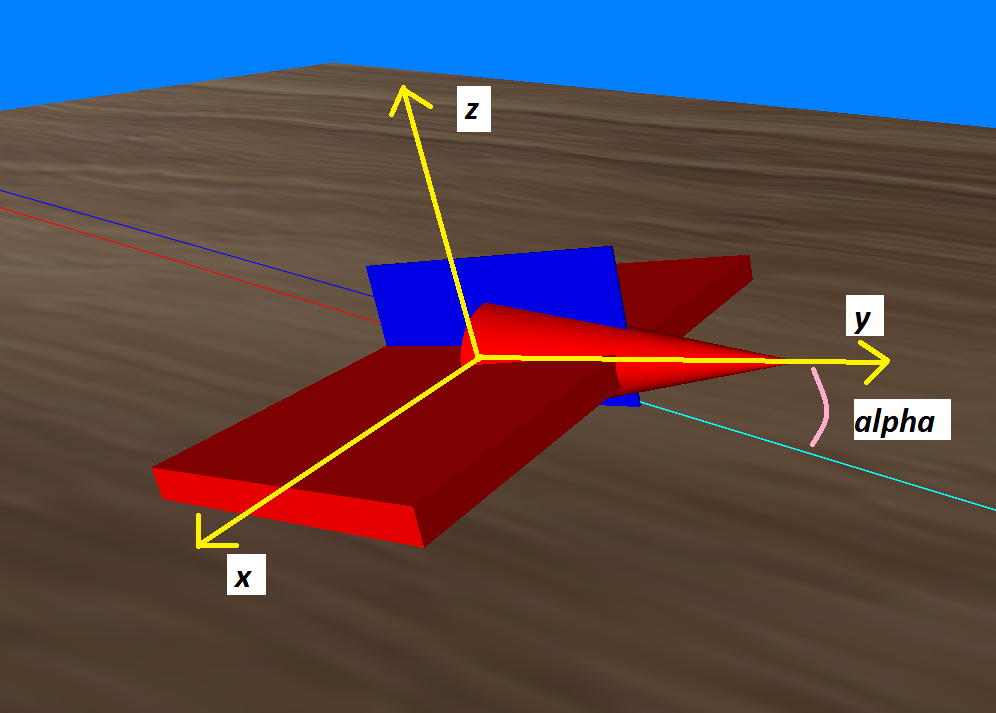
\includegraphics[trim = 0cm 0cm 0cm 0cm, clip, width=7cm]{fig1.png}
\end{center}
\caption{Frame on Aircraft}
\end{figure}

The aerodynamic force on a surface moving through the air is given as
\begin{align}
\boldsymbol{F_{\text{aero}}} = \rho A v^2 sin(\alpha)
\begin{bmatrix}
0 \\ 0 \\ 1
\end{bmatrix}
\end{align}
where
$\rho$ is the density of air,
$A$ is the area of the surface,
$v$ is the velocity of air and
$\alpha$ is the angle of attack.

The Force is a vector in 3 dimensions, with the column representing the x y and z components in the top to down order. The above $\boldsymbol{F_a}$ is a scalar multiplied by the $[0 \text{ }0 \text{ } 1]'$ vector indicating that this force only acts in the z direction in this case.

There are multiple surfaces producing this type of force, such as ailerons. The forces from all elements are as follows:

\begin{align}
\boldsymbol{F_{a0}} &= \rho A_0 v^2 sin(\alpha)
\begin{bmatrix}
0 \\ 0 \\ 1
\end{bmatrix} &\text{(force on main airframe)}
\\
\boldsymbol{F_{a1}} &= \rho A_1 v^2 sin(\alpha - u_1)
\begin{bmatrix}
0 \\ sin(u_1) \\ cos(u_1)
\end{bmatrix} &\text{(force on left aileron)}
\\
\boldsymbol{F_{a2}} &= \rho A_2 v^2 sin(\alpha - u_2)
\begin{bmatrix}
0 \\ sin(u_2) \\ cos(u_2)
\end{bmatrix} &\text{(force on right aileron)}
\\
\boldsymbol{F_{a3}} &= \rho A_3 v^2 sin(\beta - u_3)
\begin{bmatrix}
cos(u_3) \\ sin(u_3) \\ 0
\end{bmatrix} &\text{(force on rudder)}
\\
\boldsymbol{F_{a4}} &= \rho A_4 v^2 sin(\beta)
\begin{bmatrix}
1 \\ 0 \\ 0
\end{bmatrix} &\text{(force on tail)}
\end{align}

With $u_1$ the angle of left aileron, $u_2$ angle of right aileron, $u_3$ the rudder angle and $\beta$ the sideslip angle.

Adding all of these forces gives us the total aerodynamic force:
\begin{align}
\boldsymbol{F_a} &= \boldsymbol{F_{a0}} + \boldsymbol{F_{a1}} + \boldsymbol{F_{a2}} + \boldsymbol{F_{a3}} + \boldsymbol{F_{a4}}
\end{align}

Note: All of these forces are in the airplane's own frame, which do not represent lift and drag etc in the air velocity frame. If lift and drag were to be found, lift would be equal to $\boldsymbol{F_a} \cos(\alpha)$ and drag $\boldsymbol{F_a} \sin(\alpha)$.

We also know the positions of the ailerons, rudder etc. relative to the airplane frame (their distance in x y z from the center of mass of the plane). We know that the torque by any force is given by the vector cross product (with $\boldsymbol{r}$ the vector containing the relative position):

\begin{align}
\boldsymbol{\tau} = \boldsymbol{r} \times \boldsymbol{F}
\end{align}

The torques from the individual components are found in this manner (for example, the torque from the rudder is $\boldsymbol{\tau_{a3}} = \boldsymbol{r_{a3}} \times \boldsymbol{F_{a3}}$ ). To get the total aerodynamic torque, we add all of the torques together:

\begin{align}
\boldsymbol{\tau_a} &= \boldsymbol{r_{a0}} \times \boldsymbol{F_{a0}} + \boldsymbol{r_{a1}} \times \boldsymbol{F_{a1}} + \boldsymbol{r_{a2}} \times \boldsymbol{F_{a2}} + \boldsymbol{r_{a3}} \times \boldsymbol{F_{a3}} + \boldsymbol{r_{a4}} \times \boldsymbol{F_{a4}}
\end{align}

\section{Thrust, Air Friction and Total Acceleration}

The Thrust can be written as:

\begin{align}
\boldsymbol{F_t} = t_0 T_{max} 
\begin{bmatrix}
0 \\ 1 \\ 0
\end{bmatrix}
\end{align}
where $T_{max}$ is the maximum thrust, $t_0$ is a control input maintained by the pilot.

Air friction is given by 
\begin{align}
\boldsymbol{F_b} = -b_v v
\begin{bmatrix}
0 \\ 1 \\ 0
\end{bmatrix}\\
\boldsymbol{\tau_b} = -b_{\omega} \boldsymbol{\omega}
\end{align}
where $b_v$ and $b_{\omega}$ are friction constants and $\boldsymbol{\omega}$ is the angular velocity of the plane in the airplane frame.

Adding all of these forces and then dividing by airplane mass ($m$) gives us net acceleration, and adding all torques and dividing my moment of inertia gives net angular acceleration.
\begin{align}
\boldsymbol{a_{net}} &= m^{-1}(\boldsymbol{F_a} + \boldsymbol{F_t} + \boldsymbol{F_b})\\
\boldsymbol{\alpha_{net}} &= I^{-1}(\boldsymbol{\tau_a} + \boldsymbol{\tau_b})
\end{align}

Bringing these vectors into the world frame is a simple matter of applying a rotation and translation. In this document from this point onwards, the vectors $\boldsymbol{a_{net}}$ and $\boldsymbol{\alpha_{net}}$ have been rotated and translated and are now in the world frame. From now on, all other vectors are also in the world frame.

\section{Setting Up and Solving Differential Equations}
The position and velocity (both linear and angular) can be found by solving the following differential equations:

\begin{align}
\dot{x} = v \\
\dot{v} = \boldsymbol{a_{net}} \\
\dot{\theta} = \omega \\
\dot{\omega} = \boldsymbol{\alpha_{net}}
\end{align}

where $x$ is the position vector of the plane,

$v$ is the velocity vector,

$\theta$ is the angular position vector and

$\omega$ is the angular velocity.

$\dot{x}$ indicates the derivative of $x$ with respect to time ($\dot{x} = \frac{dx}{dt}$) and similarly for other values.

For any initial condition of the values of [$x$, $v$, $\theta$, $\omega$], the system of equations can be solved as
\begin{align}
x(t) = x(t_0) + \int\limits_{t_0}^{t}\dot{x}(t) dt
\end{align}
and similar relations for the other variables. Using the trapezoidal rule for the integration in $x$ and $\theta$, we have a first order solver

\begin{align}
v(t) = v(t_0) + \dot{v}(t_0)(t - t_0)\\
x(t) = x(t_0) + \frac{(\dot{x}(t) + \dot{x}(t_0))}{2} (t - t_0)\\
\omega(t) = \omega(t_0) + \dot{v}(t_0)(t - t_0)\\
\theta(t) = \theta(t_0) + \frac{(\dot{\theta}(t) + \dot{\theta}(t_0))}{2} (t - t_0)
\end{align}

Setting $t = t_0 + dt $ where $dt$ is the simulation time-step, we can find out, one by one, all future values of [$x$, $v$, $\theta$, $\omega$]. The values of $\boldsymbol{a_{net}}$ and $\boldsymbol{\alpha_{net}}$ can be changed by the pilot and can affect [$x$, $v$, $\theta$, $\omega$] and hence serve to control the airplane.

\end{document}